\exer{Recherche de connexité}
\begin{flushright}
\textit{D'après ressources Nicolas COURRIER, UPSTI.}
\end{flushright}

\section*{Introduction}
\subsection*{Définitions}

\begin{defi}{}
Un graphe non orienté $G=(S,A)$ est dit connexe si pour tout couple de sommets ($u$,$v$), il existe une chaîne reliant $u$ et $v$. 
\end{defi}


%%\bigskip
%
%Cette définition est importante car elle permet de savoir si pour n'importe quel n\oe{}ud du graphe on peut atteindre un autre n\oe{}ud de celui-ci. Cette propriété est nécessaire par exemple dans le routage de paquets via un réseau d'ordinateurs afin de déterminer si les informations peuvent transiter d'une machine à l'autre. 

\textbf{Exemples :}

\begin{center}
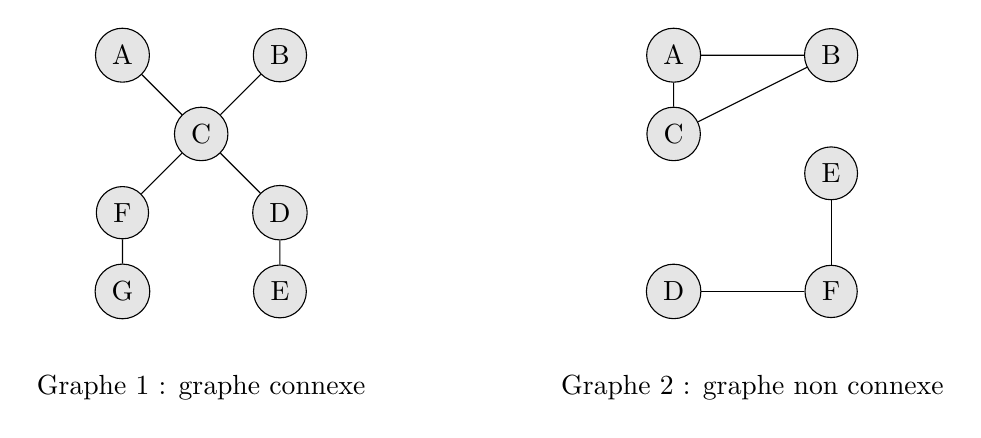
\begin{tikzpicture}[scale=1]
\tikzstyle{sommet}=[circle,draw,fill=gray!20]
\begin{scope}
\draw (0,-3.5) node[above] {Graphe 1 : graphe connexe} ;
\node[sommet] (C) at (0,0) {C};
\node[sommet] (A) at (-1,1) {A};
\node[sommet] (B) at (1,1) {B};
\node[sommet] (F) at (-1,-1) {F};
\node[sommet] (D) at (1,-1) {D};
\node[sommet] (G) at (-1,-2) {G};
\node[sommet] (E) at (1,-2) {E};
\draw (A) -- (C) -- (D) -- (E);
\draw (B) -- (C) -- (F) -- (G) ;
\end{scope}
\begin{scope}[xshift=7cm]
\draw (0,-3.5) node[above] {Graphe 2 : graphe non connexe} ;
\node[sommet] (C) at (-1,0) {C};
\node[sommet] (A) at (-1,1) {A};
\node[sommet] (B) at (1,1) {B};
\node[sommet] (F) at (1,-2) {F};
\node[sommet] (D) at (-1,-2) {D};
\node[sommet] (E) at (1,-0.5) {E};
\draw (A) -- (C) -- (B) -- (A);
\draw (D) -- (F) -- (E)  ;
\end{scope}
\end{tikzpicture}
\end{center}

%
%Le graphe 1 est connexe puisque l'on peut toujours trouver une chaîne entre tous les n\oe{}uds du graphe. Le graphe 2 n'est pas connexe car il n'y a aucune chaîne entre les sommets C et E (par exemple).



\begin{defi}{}
Un graphe qui n'est pas connexe est l'union de plusieurs sous-graphes connexes. Chacune des ces parties étant indépendantes des autres. C'est-à-dire qu'elles n'ont pas de n\oe{}uds en commun. Les sous-graphes connexes disjoints sont des \textbf{composantes connexes} du graphe.
\end{defi}

\textbf{Exemple}

\begin{center}
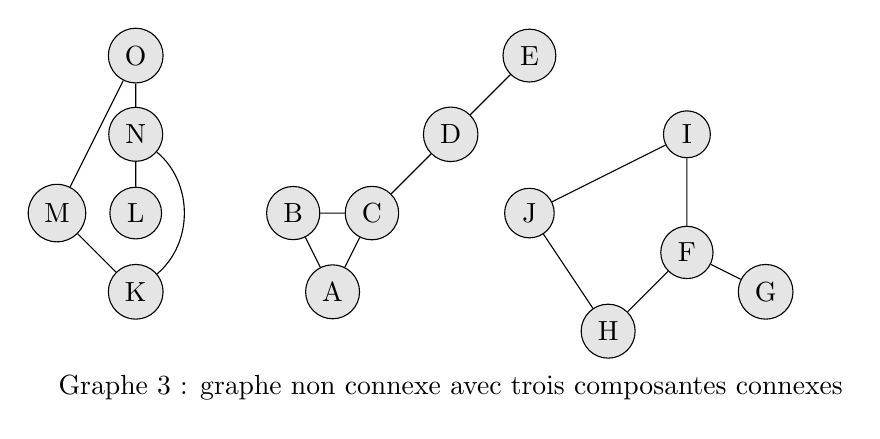
\begin{tikzpicture}[scale=1]
\tikzstyle{sommet}=[circle,draw,fill=gray!20]
\begin{scope}
\draw (0,-3.5) node[above] {Graphe 3 : graphe non connexe avec trois composantes connexes} ;
\node[sommet] (D) at (0,0) {D};
\node[sommet] (C) at (-1,-1) {C};
\node[sommet] (B) at (-2,-1) {B};
\node[sommet] (A) at (-1.5,-2) {A};
\node[sommet] (E) at (1,1) {E};
\node[sommet] (F) at (3,-1.5) {F};
\node[sommet] (G) at (4,-2) {G};
\node[sommet] (H) at (2,-2.5) {H};
\node[sommet] (I) at (3,0) {I};
\node[sommet] (J) at (1,-1) {J};
\node[sommet] (K) at (-4,-2) {K};
\node[sommet] (L) at (-4,-1) {L};
\node[sommet] (M) at (-5,-1) {M};
\node[sommet] (N) at (-4,0) {N};
\node[sommet] (O) at (-4,1) {O};
\draw (A) -- (B) -- (C) -- (D) -- (E);
\draw (A) -- (C);
\draw (F) -- (G) ;
\draw (F) -- (H) ;
\draw (F) -- (I) -- (J) -- (H);
\draw(K)--(M) --(O) -- (N) -- (L);
\draw (N) to [bend left=50] (K);
\end{scope}
\end{tikzpicture}
\end{center}


\subsection*{Préparation aux codes}

Soit le graphe suivant :
\begin{center}
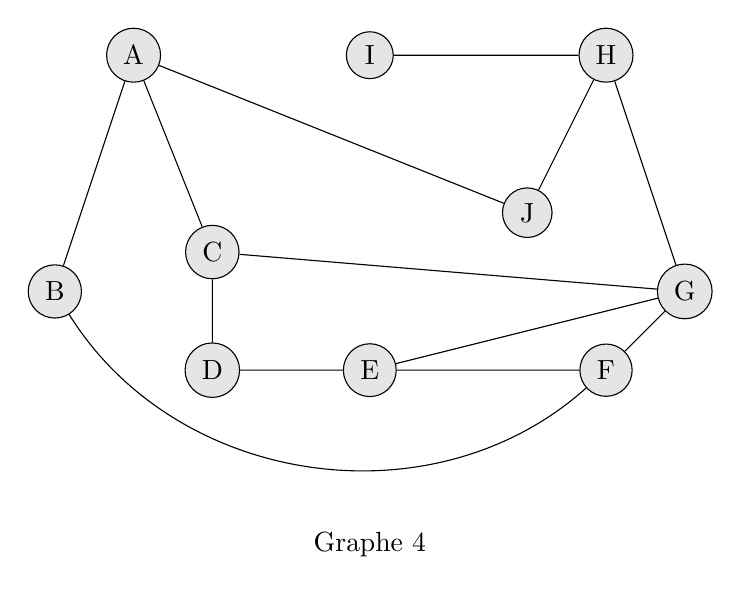
\begin{tikzpicture}[scale=1]
\tikzstyle{sommet}=[circle,draw,fill=gray!20]
\begin{scope}
\draw (0,-6.5) node[above] {Graphe 4} ;
\node[sommet] (I) at (0,0) {I};
\node[sommet] (H) at (3,0) {H};
\node[sommet] (J) at (2,-2) {J};
\node[sommet] (G) at (4,-3) {G};
\node[sommet] (F) at (3,-4) {F};
\node[sommet] (E) at (0,-4) {E};
\node[sommet] (D) at (-2,-4) {D};
\node[sommet] (C) at (-2,-2.5) {C};
\node[sommet] (A) at (-3,0) {A};
\node[sommet] (B) at (-4,-3) {B};
\draw (F) -- (G) -- (C) -- (D) -- (E) -- (F);
\draw (E) -- (G);
\draw (A) -- (C) ;
\draw (A) -- (J) -- (H) ;
\draw (I) -- (H) -- (G) ;
\draw (A) -- (B);
\draw (B) to [bend right=50] (F);
\end{scope}
\end{tikzpicture}
\end{center}

\question{Ce graphe est-il connexe ?}
\ifprof
\begin{corrige}
Depuis le n\oe{}ud A, il est possible d'atteindre l'ensemble des autres n\oe{}uds :
\begin{itemize}
\item Pour atteindre le n\oe{}ud B, la chaîne A--B est possible.
\item Pour atteindre le n\oe{}ud C, la chaîne A--C est possible.
\item Pour atteindre le n\oe{}ud D, la chaîne A--C--D est possible.
\item Pour atteindre le n\oe{}ud E, la chaîne A--C--D--E est possible.
\item Pour atteindre le n\oe{}ud F, la chaîne A--B--F est possible.
\item Pour atteindre le n\oe{}ud G, la chaîne A--C--G est possible.
\item Pour atteindre le n\oe{}ud H, la chaîne A--J--H est possible.
\item Pour atteindre le n\oe{}ud I, la chaîne A--J--H--I est possible.
\item Pour atteindre le n\oe{}ud J, la chaîne A--J est possible.
\end{itemize}

Tous les n\oe{}uds sont accessibles depuis A: \fbox{le graphe est connexe.}\\
\end{corrige}
\else
\fi

\question{Renseigner la matrice d'adjacence \texttt{mat\_adj} permettant de modéliser le graphe précédent.}
\ifprof
\begin{corrige}~\\
\begin{lstlisting}
mat_adj=[[0,1,1,0,0,0,0,0,0,1],[1,0,0,0,0,1,0,0,0,0],[1,0,0,1,0,0,1,0,0,0],
[0,0,1,0,1,0,0,0,0,0],[0,0,0,1,0,1,1,0,0,0],[0,1,0,0,1,0,1,0,0,0],
[0,0,1 ,0,1,1,0,1,0,0],[0,0,0,0,0,0,1,0,1,1],[0,0,0,0,0,0,0,1,0,0],
[1,0,0,0,0,0,0,1,0 ,0]]
\end{lstlisting}

Cela correspond à la matrice suivante:

\[ \mathbb{M}=\left(\begin{array}{cccccccccc}
0 & 1 & 1 & 0 & 0 & 0 & 0 & 0 & 0 & 1 \\ 
1 & 0 & 0 & 0 & 0 & 1 & 0 & 0 & 0 & 0 \\ 
1 & 0 & 0 & 1 & 0 & 0 & 1 & 0 & 0 & 0 \\ 
0 & 0 & 1 & 0 & 1 & 0 & 0 & 0 & 0 & 0 \\ 
0 & 0 & 0 & 1 & 0 & 1 & 1 & 0 & 0 & 0 \\ 
0 & 1 & 0 & 0 & 1 & 0 & 1 & 0 & 0 & 0 \\ 
0 & 0 & 1 & 0 & 1 & 1 & 0 & 1 & 0 & 0 \\ 
0 & 0 & 0 & 0 & 0 & 0 & 1 & 0 & 1 & 1 \\ 
0 & 0 & 0 & 0 & 0 & 0 & 0 & 1 & 0 & 0 \\ 
1 & 0 & 0 & 0 & 0 & 0 & 0 & 1 & 0 & 0
\end{array}  \right)  \]

\end{corrige}
\else
\fi


\question{Créer une fonction \texttt{verif\_symetrie(matrice)} retournant le booléen \texttt{True} si la matrice \texttt{matrice} est effectivement symétrique et \texttt{False} sinon. Vérifier ainsi que la matrice \texttt{mat\_adj} renseignée à la question précédente est bien symétrique (cela permettra de trouver d'éventuelles erreurs de rentrées d'informations).}
\ifprof
\begin{corrige}~\\
\begin{lstlisting}
def verif_symetrie(matrice):
  n=len(matrice)
  assert n==len(matrice[0]) # assertion pour vérifier que la matrice est carrée.
  for i in range(n):  # Parcours de la zone triangulaire supérieure de la matrice
    for j in range(i,n): 
      if m[i][j]!=m[j][i]: # Test de symétrie de la matrice
        return False
  return True

# Test sur la matrice définie à la question précédente
test=verif_symetrie(mat_adj)
\end{lstlisting}
\end{corrige}
\else
\fi

%
%Soit le code suivant permettant d'étiqueter les sommets du graphe :
%
%\begin{lstlisting}
%etiquettes=[chr(ord('A') + i)for i in range(len(mat_adj))]
%\end{lstlisting}
%
%\question{\`A l'aide de la commande \texttt{help}, déterminer le rôle des fonctions \texttt{ord} et \texttt{chr}. Expliquez alors ce qu'est \texttt{etiquettes}. }
%
%
Dans le but de parcourir un graphe, il est beaucoup plus simple d'identifier les sommets par des numéros (plus facile pour réaliser des boucles par exemple ou pour récupérer une ligne ou colonne de la matrice d'adjacence). Ainsi dans le cas traité, A sera le n\oe{}ud 0, B sera le n\oe{}ud 1 etc.\\

On dispose de la fonction \texttt{determination\_numero(etiquettes,nom\_noeud)} prenant comme argument la liste \texttt{etiquettes} et une chaîne de caractères \texttt{nom\_noeud}. Cette fonction retourne le numéro de n\oe{}ud associé au nom du n\oe{}ud étudié. 
On supposera que \texttt{nom\_noeud} est bien présent dans la liste  \texttt{etiquettes}.
%
%
%\question{Coder alors une fonction \texttt{determination\_numero(etiquettes,nom\_noeud)} prenant comme argument la liste \texttt{etiquettes} et une chaîne de caractères \texttt{nom\_noeud}. Cette fonction devra ainsi retourner le numéro de n\oe{}ud associé au nom du n\oe{}ud étudié. On supposera que \texttt{nom\_noeud} est bien présent dans la liste  \texttt{etiquettes}.}

Dans le but de réaliser le parcours de graphe (que ce soit en largeur ou profondeur), il est nécessaire de déterminer les voisins d'un sommet qui n'aura pas été pas été déjà découvert. On donne la liste \texttt{noeuds\_visites} contenant la liste des n\oe{}uds déjà découverts (ou visités).\\

\question{Créer une fonction \texttt{recherche\_voisins(mat\_adj,noeuds\_visites,noeud)} ayant comme arguments la matrice d'adjacence, la liste des n\oe{}uds déjà découverts et le n\oe{}ud \texttt{noeud} dont on cherche les voisins encore non visités. Cette fonction renverra ainsi la liste des n\oe{}uds voisins non visités. On précise que dans cette fonction les sommets (ou n\oe{}uds) sont identifiés par leur numéro. Ainsi, par exemple \texttt{recherche\_voisins(mat\_adj,[0,1,3],2)} doit renvoyer [6]. En effet, on cherche ici les sommets voisins de C parmi ceux non visités. Les n\oe{}uds déjà visités dans cet exemple sont A, B et D. Le sommet G est le seul voisin de C non visité.}
\ifprof
\begin{corrige}~\\
\begin{lstlisting}
def recherche_voisins(mat_adj,noeuds_visites,noeud):
    return [i for i in range(len(mat_adj)) if mat_adj[noeud][i]!=0  \
    and i not in noeuds_visites]
\end{lstlisting}
\end{corrige}
\else
\fi

\section*{Parcours en largeur}

%\question{Réalisez une fonction \texttt{listes\_adjacences(m)} prenant en argument la matrice \texttt{m} et renvoyant une liste \texttt{adj} composée les différentes listes d'adjacences des n\oe{}uds classées dans l'ordre. Dans notre exemple, on trouvera donc : \\
%\texttt{adj=[[1,2,9],[0,5],[0,3,6],[2,4],[3,5,6],[1,4,6],[2,4,5,7],[6,8,9],[7],[0,7]]}
%
%
%\begin{lstlisting}
%def connexion(m):
%    n=len(m)
%    adj=[]
%    for i in range(n):
%        temp=[]
%        for j in range(n):
%            if m[i][j]!=0:
%                temp.append(j)
%        adj.append(temp)
%    return adj
%\end{lstlisting}

\question{Réaliser \og à la main \fg{} le parcours en largeur du graphe proposé en partant du n\oe{}ud A et dessinez l'arbre ainsi obtenu.}
\ifprof
\begin{corrige}
\begin{center}
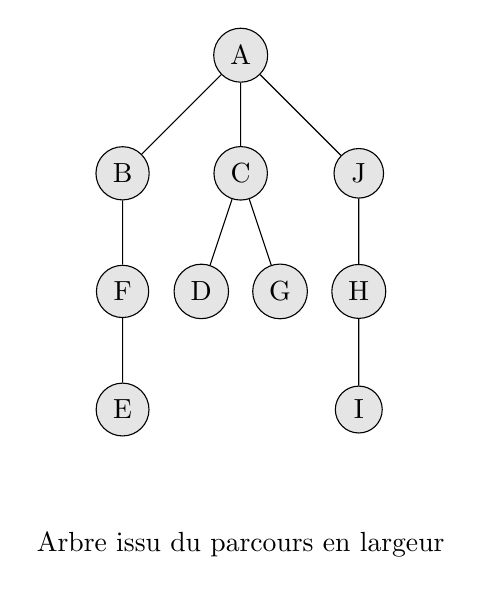
\begin{tikzpicture}[scale=1]
\tikzstyle{sommet}=[circle,draw,fill=gray!20]
\begin{scope}
\draw (0,-6.5) node[above] {Arbre issu du parcours en largeur} ;
\node[sommet] (A) at (0,0) {A};
\node[sommet] (B) at (-1.5,-1.5) {B};
\node[sommet] (C) at (0,-1.5) {C};
\node[sommet] (J) at (1.5,-1.5) {J};
\node[sommet] (F) at (-1.5,-3) {F};
\node[sommet] (D) at (-0.5,-3) {D};
\node[sommet] (G) at (0.5,-3) {G};
\node[sommet] (H) at (1.5,-3) {H};
\node[sommet] (E) at (-1.5,-4.5) {E};
\node[sommet] (I) at (1.5,-4.5) {I};
\draw (A) -- (B) -- (F) -- (E) ;
\draw (A) -- (C) -- (D);
\draw (C) -- (G) ;
\draw (A) -- (J) -- (H) -- (I) ;
\end{scope}
\end{tikzpicture}
\end{center}
\end{corrige}
\else
\fi

%\question{Réaliser \og à la main \fg{} le parcours en profondeur du graphe proposé en partant du n\oe{}ud A et dessinez l'arbre ainsi obtenu.}
%\ifprof
%\begin{corrige}
%\begin{lstlisting}
%
%\end{lstlisting}
%\end{corrige}
%\else
%\fi


%\question{Cet arbre est-il connexe ?}

\begin{defi}{}Lors d'un parcours en largeur ou profondeur d'un graphe, si l'arbre de parcours obtenu est couvrant -- c'est-à-dire  que l'arbre contient l'ensemble des n\oe{}uds du graphe -- alors le graphe est connexe.
\end{defi}
%
%Le principe de l'algorithme de parcours en longueur se base sur la notion de file. Le pseudo-code permettant de réaliser le parcours en largeur d'un graphe est le suivant :
%
%\begin{algorithm}[H]
%\SetAlgoLined
% \textbf{Initialisation}\;
% Initialiser la liste \texttt{file} avec le n\oe{}ud départ \;
% Initialiser la liste \texttt{noeuds\_visites} avec le n\oe{}ud départ \;
% \Tq{\texttt{file} n'est pas vide}{
%  noeud\_courant $\leftarrow$ tête(\texttt{file}) (Penser donc à éliminer ce n\oe{}ud de la file)\;
%  \Pour{chacun des voisins $v$ de noeud\_courant non visité}{
%  	Ajouter $v$ à la liste \texttt{noeuds\_visites}\;
%  	Enfiler $v$ à la fin de la liste \texttt{file}}
%   }
%   \Return {\texttt{noeuds\_visites}}
% \caption{Algorithme de parcours de graphe en largeur}
%\end{algorithm}
%~~\\

\question{Réaliser une fonction \texttt{parcours\_largeur\_graphe(mat\_adj,depart,etiquettes)} prenant en argument la matrice d'adjacence du graphe, la liste \texttt{etiquettes} et le n\oe{}ud de départ (avec son nom et non pas son numéro par exemple \texttt{parcours\_largeur\_graphe(mat\_adj,'A',etiquettes)}. Cette fonction devrait renvoyer la liste des n\oe{}uds suite au parcours en largeur du graphe.}
\ifprof
\begin{corrige}~\\
\begin{lstlisting}
def parcours_largeur_graphe(mat_adj,depart,etiquettes):
    # Récupération du numéro de noeud de départ
    num_noeud_depart=determination_numero(etiquettes,depart)
    # Initialisation de la file avec le premier noeud à visiter 
    file=[num_noeud_depart] 
    # Initialisation de la variable qui contiendra les numéros de noeuds visités, 
    # on commence par le noeud départ
    noeuds_visites=[num_noeud_depart] 
    while len(file) != 0:
    	# Recupération du numéro du noeud courant
        noeud_courant=file[0] 
        # Elimination de noeud de la liste file
        file[0:1]=[] 
        # Recherche des voisins non découverts
        voisins_non_visites=recherche_voisins(mat_adj,noeuds_visites,noeud_courant) 
		# Pour tous les noeuds voisin du noeud courant non visités...        
        for v in voisins_non_visites: 
        			# ... on l'ajoute aux noeuds visités ...
                noeuds_visites.append(v) 
                # ... et à la file d'étude.
                file.append(v) 
    return [etiquettes[noeuds_visites[i]] for i in range(len(noeuds_visites))]

\end{lstlisting}
\end{corrige}
\else
\fi


\question{Modifier le code précédent pour que la fonction \texttt{parcours\_largeur\_graphe} retourne en plus de la liste des n\oe{}uds visités : }
\textit{\begin{itemize}
\item la matrice d'adjacence du graphe de parcours obtenu;
\item la liste \texttt{provenance} contenant le numéro du n\oe{}ud  \og père \fg{} ou \og origine \fg{} dont est issu un n\oe{}ud découvert. L'origine du sommet de départ est lui-même. Par exemple en partant du n\oe{}ud A, on doit obtenir la liste \texttt{provenance}=[0,0,0,2,5,1,2,9,7,0]. En effet, lors du processus du parcours, le n\oe{}ud B a pour origine le n\oe{}ud A, le n\oe{}ud C également, le n\oe{}ud D a pour n\oe{}ud père C etc. Si un n\oe{}ud n'a pas été découvert alors son origine sera \texttt{None}.
\end{itemize}}
\ifprof
\begin{corrige}
\begin{lstlisting}
def parcours_largeur_graphe(mat_adj,depart,etiquettes):
	# Récupération du numéro de noeud de départ
    num_noeud_depart=determination_numero(etiquettes,depart) 
    # Initialisation de la file avec le premier noeud à visiter
    file=[num_noeud_depart]
    # Initialisation de la variable qui contiendra les numéros de noeuds visités, 
    # on commence par le noeud départ 
    noeuds_visites=[num_noeud_depart] 
    n=len(mat_adj)
    # Initialisation  de la liste provenance
    provenance=[None]*n 
    provenance[num_noeud_depart]=num_noeud_depart
    # Initialisation de la matrice d'adjacence de l'arbre obtenu suite au parcours effectué.
    mat_arbre=[[0]*n for i in range(n)] 
    while len(file) != 0:
    		# Recupération du numéro du noeud courant
        noeud_courant=file[0] 
        # Elimination de noeud de la liste file
        file[0:1]=[] 
        # Recherhce des voisins non découverts
        voisins_non_visites=recherche_voisins(mat_adj,noeuds_visites,noeud_courant) 
        # Pour tous les noeuds voisin du noeud courant non visités...
        for v in voisins_non_visites: 
        		# ... on l'ajoute aux noeuds visités ...
            noeuds_visites.append(v) 
            # ... et à la file d'étude.
            file.append(v) 
            # Mise à jour de la liste provenance
            provenance[v]=noeud_courant 
            # Mise à jour de la matrice d'adjacence de l'arbre obtenu
            mat_arbre[noeud_courant][v],mat_arbre[v][noeud_courant]=1,1 
    return [etiquettes[noeuds_visites[i]] for i in range(len(noeuds_visites))],
    mat_arbre,provenance
\end{lstlisting}
\end{corrige}
\else
\fi




\question{D'après la \textbf{Définition 3}, comment peut-on savoir si le graphe est connexe ?}
\ifprof
\begin{corrige}
Le graphe est connexe à condition que la liste des n\oe{}uds parcourus contiennent tous les n\oe{}uds du graphe. Autrement dit, on peut tester si le graphe est connexe en faisant
\begin{lstlisting}
liste_noeuds,mat_arbre,provenance= parcours_largeur_graphe(mat_adj,'A',etiquettes)
if len(liste_noeuds)==len(mat_adj):
    print("Le graphe est connexe")
else:
   print("Le graphe n'est pas connexe")
\end{lstlisting}
\end{corrige}
\else
\fi

La ligne de code suivante a été tapée, avec \texttt{depart} un n\oe{}ud du graphe :

\begin{lstlisting}
liste_noeuds,mat_arbre,provenance= \
parcours_largeur_graphe(mat_adj,depart,etiquettes) 
\end{lstlisting}


\question{\`A l'aide d'une fonction \texttt{restitution\_parcours(provenance,etiquettes,depart,arrivee} établir la chaîne permettant d'aller du n\oe{}ud \texttt{depart} au n\oe{}ud arrivee.}
\ifprof
\begin{corrige}~\\
\begin{lstlisting}
def restitution_parcours(provenance,etiquettes,depart,arrivee):
    s =""
    num_depart=determination_numero(etiquettes,depart)
    num_arrivee=determination_numero(etiquettes,arrivee)
    num=num_arrivee
    while num != num_depart:
        s =' '+ etiquettes[num] + s
        num = provenance[num]
    return etiquettes[num_depart] + s
\end{lstlisting}
\end{corrige}
\else
\fi


\begin{defi}{}
Le parcours en largeur permet de trouver le chemin le plus court (si les arêtes ne sont pas pondérées) entre deux sommets.
\end{defi}


\section*{Parcours en profondeur}

%\question{Réaliser le codage \og à la main \fg{} récursif du parcours en profondeur du graphe étudié en partant du point A. Quand plusieurs possibilités se présentent à vous, vous choisirez d'explorer le n\oe{}ud le mieux classé dans l'ordre alphabétique.}

\question{Réaliser le codage \og à la main \fg{}  du parcours en profondeur du graphe étudié en partant du point A. Quand plusieurs possibilités se présentent à vous, vous choisirez d'explorer le n\oe{}ud le mieux classé dans l'ordre alphabétique.}
\ifprof
\begin{corrige}~\\
\begin{center}
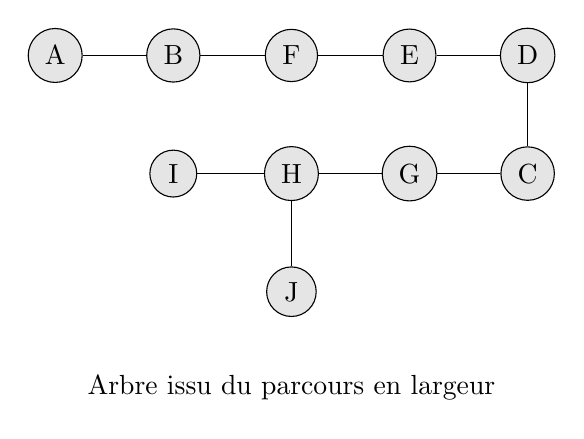
\begin{tikzpicture}[scale=1]
\tikzstyle{sommet}=[circle,draw,fill=gray!20]
\begin{scope}
\draw (-3,-4.5) node[above] {Arbre issu du parcours en largeur} ;
\node[sommet] (A) at (-6,0) {A};
\node[sommet] (B) at (-4.5,0) {B};
\node[sommet] (F) at (-3,0) {F};
\node[sommet] (E) at (-1.5,0) {E};
\node[sommet] (D) at (0,0) {D};
\node[sommet] (C) at (0,-1.5) {C};
\node[sommet] (G) at (-1.5,-1.5) {G};
\node[sommet] (H) at (-3,-1.5) {H};
\node[sommet] (I) at (-4.5,-1.5) {I};
\node[sommet] (J) at (-3,-3) {J};
\draw (A) -- (B) -- (F) -- (E)  -- (D) -- (C) -- (G) -- (H) -- (I);
\draw (H) -- (J);
\end{scope}
\end{tikzpicture}
\end{center}
\end{corrige}
\else
\fi


%Le pseudo-code du parcours en profondeur d'un graphe est le suivant :\\
%
%
%\begin{algorithm}[H]
%\SetAlgoLined
% \textbf{Initialisation}\;
% Initialiser la liste \texttt{noeuds\_visites} avec le n\oe{}ud départ \;
%  	Visiter(noeud\_depart,noeuds\_visites)\;
%   \Return {\texttt{noeuds\_visites}}
% \caption{Algorithme de parcours de graphe en profondeur récursif}
%\end{algorithm}
%
%\begin{algorithm}[H]
%\SetAlgoLined
%\Si{ u n'est pas dans la liste noeuds\_visites}{
% Ajouter $u$ à la liste noeuds\_visites\;}
%  \Pour{chaque sommet v voisin non visité de u}{
%  	Visiter(v,noeuds\_visites)\;
%  	}
% \caption{Fonction récursive Visiter(u,noeuds\_visites)}
%\end{algorithm}
%~~\\

\question{Réaliser une fonction \texttt{parcours\_profondeur\_graphe(mat\_adj,depart,etiquettes)} prenant en argument la matrice d'adjacence du graphe, la liste \texttt{etiquettes} et le n\oe{}ud de départ (avec son nom et non pas son numéro par exemple \texttt{parcours\_largeur\_graphe(mat\_adj,'A',etiquettes)}. Cette fonction devrait renvoyer la liste des n\oe{}uds suite au parcours en profondeur du graphe.}
\ifprof
\begin{corrige}~\\
\begin{lstlisting}
def parcours_profondeur_graphe(mat_adj,depart,etiquettes):
    num_noeud_depart=determination_numero(etiquettes,depart) # Récupération du numéro de noeud de départ
    noeuds_visites=[num_noeud_depart]
    visiter(num_noeud_depart,noeuds_visites)
    return [etiquettes[noeuds_visites[i]] for i in range(len(noeuds_visites))]
    
def visiter(noeud,noeuds_visites):
    if noeud not in noeuds_visites:
        noeuds_visites.append(noeud)
    voisins_non_visites=recherche_voisins(mat_adj,noeuds_visites,noeud)
    for v in voisins_non_visites:
        visiter(v,noeuds_visites)

\end{lstlisting}
\end{corrige}
\else
\fi
      
\question{Modifier la fonction \texttt{visiter} et parcours\_profondeur\_graphe de façon à retourner également :}
 \textit{ \begin{itemize}
\item la matrice d'adjacence du graphe de parcours obtenu;
\item la liste \texttt{provenance} contenant le numéro du n\oe{}ud  \og père \fg{} ou \og origine \fg{} dont est issu un n\oe{}ud découvert. L'origine du sommet de départ est lui-même. Par exemple en partant du n\oe{}ud A, on doit obtenir la liste \texttt{provenance}=[0, 0, 3, 4, 5, 1, 2, 6, 7, 7]. En effet, lors du processus du parcours, le n\oe{}ud B a pour origine le n\oe{}ud A, le n\oe{}ud C a pour n\oe{}ud père D, etc. Si un n\oe{}ud n'a pas été découvert alors son origine sera \texttt{None}.
\end{itemize}}
\ifprof
\begin{corrige}~\\
\begin{lstlisting}
def parcours_profondeur_graphe(mat_adj,depart,etiquettes):
	# Récupération du numéro de noeud de départ
    num_noeud_depart=determination_numero(etiquettes,depart) 
    n=len(mat_adj)
    provenance=[None]*n
    provenance[num_noeud_depart]=num_noeud_depart
    noeuds_visites=[num_noeud_depart]
    mat_arbre=[[0]*n for i in range(n)]
    visiter(num_noeud_depart,noeuds_visites,provenance,mat_arbre,num_noeud_depart)
    return [etiquettes[noeuds_visites[i]] for i in range(len(noeuds_visites))],
    mat_arbre,provenance
    
def visiter(noeud,noeuds_visites,provenance,mat_arbre,noeud_pere):
    if noeud not in noeuds_visites:
        noeuds_visites.append(noeud)
        provenance[noeud]=noeud_pere
        mat_arbre[noeud][noeud_pere],mat_arbre[noeud_pere][noeud_pere]=1,1
    voisins_non_visites=recherche_voisins(mat_adj,noeuds_visites,noeud)
    for v in voisins_non_visites:
        visiter(v,noeuds_visites,provenance,mat_arbre,noeud)
\end{lstlisting}
\end{corrige}
\else
\fi
 
\section*{Optimisation en temps}

\subsection*{Parcours en largeur : Utilisation des files}

Dans cette section, on va chercher à optimiser un code de parcours en largeur d'un graphe. Le premier graphe proposé est composé de $2000$ n\oe{}uds, le second de $5000$. Pour réaliser cette partie, un fichier \og codes\_parcours\_graphe.py \fg{} et deux fichiers contenant les matrices d'adjacence des graphes sont à votre disposition : \og graphe\_2000.txt \fg{} et  \og graphe\_5000.txt \fg{}.\\

\question{Dans un fichier principal \og main.py \fg{} importer via la commande \texttt{from ... import}, l'ensemble des fonctions du fichier  \og codes\_parcours\_graphe.py \fg{}}
\ifprof
\begin{corrige}
\begin{lstlisting}

\end{lstlisting}
\end{corrige}
\else
\fi

\question{Dans le fichier principal, coder l'ouverture et la lecture du fichier \og graphe\_2000.txt \fg{}. Stocker la matrice d'adjacence ainsi obtenue dans une variable \texttt{mat\_adj}. Si besoin consulter le fonctionnement de la commande \texttt{eval} (\texttt{help(eval)}).}
\ifprof
\begin{corrige}
\begin{lstlisting}

\end{lstlisting}
\end{corrige}
\else
\fi

Sachant que la fonction \texttt{time()} de la bibliothèque \texttt{time} permet de prendre la mesure du temps à l'instant $t$, pour estimer la durée d'une action, il faut donc prendre la différence entre deux points de mesures, comme sur l'exemple ci-dessous :
\begin{lstlisting}
t1=time.time()
Action quelconque
...
t2=time.time()
duree=t2-t1
 \end{lstlisting}
 
\textbf{Remarque:} sur les versions plus récentes de Python, la fonction \texttt{time()} a été supprimée au profit de \texttt{process\_time()}.\\

\question{ \`A l'aide de cette explication, de la spécification et des commentaires présents dans le code \texttt{parcours\_largeur\_graphe1}, expliquer le rôle de celui-ci et les informations que l'on a en retour.}
\ifprof
\begin{corrige}
\begin{lstlisting}

\end{lstlisting}
\end{corrige}
\else
\fi

\question{Dans le fichier principal, importer le module \texttt{time} et réaliser le parcours de graphe à l'aide de la fonction \texttt{parcours\_largeur\_graphe1}. Mesurer le temps total d'exécution ainsi que le temps d'exécution des différentes opérations effectuées lors de l'appel à cette fonction. Afficher ces temps à l'écran. }
\ifprof
\begin{corrige}
\begin{lstlisting}

\end{lstlisting}
\end{corrige}
\else
\fi

La durée totale du code est de 32.68 s, la gestion de la file prend  0.01 s, la gestion de la liste \texttt{noeuds\_visites}  0.001 s et la recherche de voisins non visités 32.65 s.\\
 
\question{Sur quel paramètre peut-on essayer de jouer pour gagner du temps ?}

\ifprof
\begin{corrige}
\begin{lstlisting}

\end{lstlisting}
\end{corrige}
\else
\fi
\question{Quelle est la différence principale entre le code \texttt{parcours\_largeur\_graphe1} et le code \texttt{parcours\_largeur\_graphe2} ?}
\ifprof
\begin{corrige}
\begin{lstlisting}

\end{lstlisting}
\end{corrige}
\else
\fi



\question{Dans le fichier principal, réaliser maintenant le parcours de graphe à l'aide de la fonction \texttt{parcours\_largeur\_graphe2} . Mesurer le temps total d'exécution ainsi que le temps d'exécution des différentes opérations effectuées lors de l'appel à cette fonction. Afficher ces temps à l'écran. Entre la phase de recherche des voisins d'un n\oe{}ud et la phase de test pour savoir si un voisin de ce n\oe{}ud a déjà été découvert, quelle est l'étape la plus longue ? }
\ifprof
\begin{corrige}
\begin{lstlisting}

\end{lstlisting}
\end{corrige}
\else
\fi

\question{Justifier alors le fonctionnement du code \texttt{parcours\_largeur\_graphe3}.}
\ifprof
\begin{corrige}
\begin{lstlisting}

\end{lstlisting}
\end{corrige}
\else
\fi

\question{Dans votre fichier principal, réaliser maintenant le parcours de graphe à l'aide de la fonction\texttt{parcours\_largeur\_graphe3} . Conclure sur la stratégie adoptée.}
\ifprof
\begin{corrige}
\begin{lstlisting}

\end{lstlisting}
\end{corrige}
\else
\fi

On a pu constater que l'utilisation d'une liste de taille connue et définie à l'avance était plus efficace que la manipulation de celle-ci (ajout d'élément ou recherche dans celle-ci). Fort de cette constatation, on peut remarquer que dans les codes proposés, la liste \texttt{file} subit des modifications de taille au fur et à mesure des boucles. Le principe de fonctionnement d'une file s'appuie sur le principe du premier arrivé, premier sorti (FIFO : First in, First out). C'est-à-dire que les nouveaux éléments à traiter sont stocker en fin de file et ceux qui vont être traités sont en début de file. Exactement comme une file d'attente à la caisse d'un supermarché.

Le principe d'une file est de stocker les nouveaux éléments en fin de file et de stocker un élément dans une variable tout en le retirant du début de file pour poursuivre l'algorithme.\\

\question{On peut encore chercher à améliorer l'efficacité du code en utilisant la bibliothèque \texttt{collections} et la fonction \texttt{deque}. En effet, celle-ci est spécialement dédiée à la construction de piles et de files. Réaliser le code suivant :
\begin{itemize}
\item créer une liste de nombres aléatoires de 100000 éléments;
\item créer à l'aide de cette liste, la file correspondante à l'aide de la fonction \texttt{deque};
\item dans deux boucles \texttt{for} distinctes de 100000 itérations chacune, simuler la récupération du premier élément de la liste ou de la file ainsi que la suppression de celui-ci dans cette même liste ou file. (Ce qui est fait lors du parcours de graphe). Utiliser pour cela l'annexe proposée sur le module \texttt{collections.deque}; 
\item mesurer les temps d'exécution de ces deux boucles.
\end{itemize}
Conclure.}
\ifprof
\begin{corrige}
\begin{lstlisting}

\end{lstlisting}
\end{corrige}
\else
\fi
 
\question{Proposer alors un code optimisé (en partie en réalité) du parcours de graphe en largeur.}
\ifprof
\begin{corrige}
\begin{lstlisting}

\end{lstlisting}
\end{corrige}
\else
\fi

\question{Le graphe de 200 sommets proposés est-il connexe ?}
\ifprof
\begin{corrige}
\begin{lstlisting}

\end{lstlisting}
\end{corrige}
\else
\fi

\question{Si votre ordinateur le permet, comparer les durées d'exécution des codes \texttt{parcours\_largeur\_graphe1} et celui que vous avez proposé avec le graphe composé de $5000$ n\oe{}uds.}
\ifprof
\begin{corrige}
\begin{lstlisting}

\end{lstlisting}
\end{corrige}
\else
\fi

\subsection*{Parcours en profondeur : Utilisation des piles}

Vous venez de réaliser l'optimisation d'un code de parcours en largeur d'un graphe relativement "simpliste" (au sens où il ne renseigne que sur les n\oe{}uds qui ont été découverts lors du parcours). L'utilisation d'une file avec le module \texttt{collections.deque} et une amélioration de la structure du code ont permis d'optimiser en bonne partie le temps de calcul.\\


\question{Reprendre votre code de parcours en profondeur d'un graphe et l'optimiser. Bien entendu comme pour la partie précédente, il ne renverra que l'information des n\oe{}uds découverts.}
\ifprof
\begin{corrige}
\begin{lstlisting}

\end{lstlisting}
\end{corrige}
\else
\fi

\question{Mesurer le temps nécessaire pour parcourir le graphe de $2000$ n\oe{}uds proposé dans le fichier \og graphe\_2000.txt \fg{}. Que constate-t-on ?}
\ifprof
\begin{corrige}
\begin{lstlisting}

\end{lstlisting}
\end{corrige}
\else
\fi
% 
% Afin de palier à ce problème, on se propose d'établir un algorithme de parcours en profondeur itératif se basant sur la simulation de la pile de récursivité. Le pseudo-code de cet algorithme est le suivant :\\
% 
% \begin{algorithm}[H]
%\SetAlgoLined
%\textbf{Initialisation}\;
%Initialiser la liste des n\oe{}uds découverts (ou visités)\;
%Initialiser la pile d'appel avec le n\oe{}ud de départ\;
%\Tq{la pile n'est pas vide}{
%Récupérer le n\oe{}ud courant et le supprimer de la pile d'appel\;
%Marquer ce n\oe{}ud comme étant visité\;
%Rechercher les n\oe{}uds voisins non visités et les ajouter à la pile\;
%  	}
%\Return la liste des n\oe{}uds découverts
%\caption{Algorithme de parcours de graphe en profondeur itératif}
%\end{algorithm}
%~~\\

\question{Coder cet algorithme à l'aide du module \texttt{collections.deque} et mesurer le temps d'exécution nécessaire pour le graphe à $2000$ n\oe{}uds.}
\ifprof
\begin{corrige}
\begin{lstlisting}

\end{lstlisting}
\end{corrige}
\else
\fi


 
%\question{Mesurer la durée d'exécution complète du code proposé
%
%\question{\`A l'aide de la fonction \texttt{time()} de la bibliothèque \texttt{time} estimez le temps nécessaire pour que cet algorithme de parcours en largeur se fasse sur le graphe proposé à $2000$ n\oe{}uds.}
%
%\begin{lstlisting}
%tic=time.time()
%liste_noeuds=parcours_largeur_graphe(mat_adj,0)
%toc=time.time()
%duree=toc-tic
%print("Durée du code initial :",duree) 
% \end{lstlisting}
%
%La temps nécessaire pour exécuter ce code est d'environ 30 secondes.

%On va chercher à optimiser ce code. La première piste facilement exploitable est celle de la recherche des voisins non visités. En effet, plutôt que d'obtenir en une seule fois la liste des voisins d'un sommet qui n'ont pas encore été découverts : 
%\begin{lstlisting}
%voisins_non_visites=[i for i in range(len(mat_adj)) if mat_adj[noeud_courant][i]!=0 and i not in noeuds_visites] 
% \end{lstlisting}
%il peut être plus efficace de d'abord trouver l'ensemble des voisins d'un n\oe{}ud et ensuite à l'aide d'un test dans la boucle \texttt{for} de vérifier si le n\oe{}ud voisin testé a été déjà découvert auparavant.
%
%Ainsi nous passerions de la structure suivante :
%\begin{lstlisting}
%voisins_non_visites=[i for i in range(len(mat_adj)) if mat_adj[noeud_courant][i]!=0 and i not in noeuds_visites] 
%for v in voisins_non_visites: 
%    noeuds_visites.append(v)
%    file.append(v)
% \end{lstlisting}
% à la structure :
% \begin{lstlisting}
%voisins=[i for i in range(len(mat_adj)) if mat_adj[noeud_courant][i]!=0] 
%for v in voisins: 
%    if v not in noeuds_visites
%        noeuds_visites.append(v)
%        file.append(v)
% \end{lstlisting}
%
%\question{\'Ecrire une fonction \texttt{parcours\_largeur\_graphe\_optim1(mat\_adj,depart)} en tenant compte de cette modification et faire la mesure du temps nécessaire pour que l'algorithme s'exécute.}
